% REMEMBER: You must not plagiarise anything in your report. Be extremely careful.

\documentclass{l4proj}

    
%
% put any additional packages here
%

\begin{document}

%==============================================================================
%% METADATA
\title{3D Animation of Barendregt's Lambda Cube}
\author{Hugo Findlay}
\date{September 25th, 2023}

\maketitle

%==============================================================================
%% ABSTRACT
\begin{abstract}
    The goal of this project was to create a website with an animated three dimensional representation of the lambda cube, that could be navigated by a user to help them learn about it.
    
\end{abstract}

%==============================================================================

% EDUCATION REUSE CONSENT FORM
% If you consent to your project being shown to future students for educational purposes
% then insert your name and the date below to  sign the education use form that appears in the front of the document. 
% You must explicitly give consent if you wish to do so.
% If you sign, your project may be included in the Hall of Fame if it scores particularly highly.
%
% Please note that you are under no obligation to sign 
% this declaration, but doing so would help future students.
%
\def\consentname {Hugo Findlay} % your full name
\def\consentdate {14 February 2024} % the date you agree
%
\educationalconsent


%==============================================================================
\tableofcontents

%==============================================================================
%% Notes on formatting
%==============================================================================
% The first page, abstract and table of contents are numbered using Roman numerals and are not
% included in the page count. 
%
% From now on pages are numbered
% using Arabic numerals. Therefore, immediately after the first call to \chapter we need the call
% \pagenumbering{arabic} and this should be called once only in the document. 
%
% Do not alter the bibliography style.
%
% The first Chapter should then be on page 1. You are allowed 40 pages for a 40 credit project and 30 pages for a 
% 20 credit report. This includes everything numbered in Arabic numerals (excluding front matter) up
% to but excluding the appendices and bibliography.
%
% You must not alter text size (it is currently 10pt) or alter margins or spacing.
%
%
%==================================================================================================================================
%
% IMPORTANT
% The chapter headings here are **suggestions**. You don't have to follow this model if
% it doesn't fit your project. Every project should have an introduction and conclusion,
% however. 
%
%==================================================================================================================================
\chapter{Introduction}

% reset page numbering. Don't remove this!
\pagenumbering{arabic} 

This chapter talks about the motivation behind the project and its aims.  There then follows an outline of how the rest of the paper is structured

\section{Motivation}

As of this April, it will have been thirty-three years since the Lambda Cube was first described by Henk Barendregt.  However, it has been an existence marked by obscurity; having little presence on the internet, and rarely being fully depicted.  The motivation of this project was to bring the cube to light and make it easier for students to learn about it.

The web format offers the capability to represent the cube as a truly three dimensional experience. This means we are able to show the interconnected nature of the systems which make up the lambda cube in a more relatable and visceral way than a simple paper explanation.  The interactive nature of the website will offer the user to learn by doing rather than just by reading.

There is also a difficulty in locating sources about the systems which comprise the cube.  Much of this is because the field of lambda calculus is diverse and old, and interacts with many other fields of mathematics and computing.  A result of this is a wide range of sources, with many using different terminology to describe identical concepts.

There was also a need for a website like this in the University, for the Theory of Computation module, as there are currently few good sources inside the university for this.

\section{Aims}

The aims which were identified before the start of the project were: 
\begin{itemize}
    \item
    \textbf{to make learning about the lambda cube more accessible} by giving concise, consistent and relevant information about each system.  To do this I would have to write about the theory behind each type system as well as explaining the differences in the syntax, beta reduction rules and typing rules in each system or corner of the cube.

    \item
    \textbf{to properly take advantage of the interactivity of the web medium}, as the common explanations around today are mostly in the same format as when the theory was first introduced in the early 1990's.  By allowing the website's user to navigate around a three dimensional representation of the cube, they should be better able to grasp the interconnectedness of the systems, and be more engaged by the learning process by choosing the order in which they learn about the systems.

    \item
    \textbf{to collate useful sources about the systems comprising the lambda cube} as there is not a commonly or easily available list of reliable textbooks or papers about each system.  In order for the website to be a useful educational resource, I would have to find appropriate and up to date sources for each combination of type systems in the cube, and display them in a clear and consistent manner.
\end{itemize}

\section{Outline}

The remainder of this paper explores and evaluates how I approached these aims, and how successful I was in achieving them.

\begin{itemize}
    \item
    \textbf{Background} focuses on the lambda cube's extant representations online and in paper,  evaluating their merits and considering their weaknesses, learning what ideas can be taken from them.
    \item
    \textbf{Requirements} talks about the specific  of the website at the start of the project and how they were derived
    \item
    \textbf{Design} details the research I undertook to select the technology, outlines the architecture and implementation I used, and how I conducted my own research into the Lambda Cube to find appropriate information and sources
    \item
    \textbf{Implementation} covers the specific implementation used to address each requirements, and the issues which arose during the development process
    \item
    \textbf{Evaluation} discusses the user studies, including details about their structure, results, the actions I took to implement the feedback and how effective the evaluation process was.
    \item
    \textbf{Conclusion} retrospects the project as a whole and considers how effectively I achieved the aims outlined in the first chapter, and the specific requirements laid out in chapter three.
    
\end{itemize}

%==================================================================================================================================
\chapter{Background and related work}

The concept of the lambda cube was first introduced in the 1991 article "an introduction to generalised type systems" in the Journal of Functional Programming by Henk Barendregt.  The first half of the article explains the lambda cube, and the second half goes on to talk about Propositions as types, which is related to but distinct from the lambda calculi which my project discusses.

As is is the first place where the concept of the lambda calculus was introduced,.  The article includes many proofs and exercises to help explain the concept, as well as using some analogies to help explain difficult concepts.

For all of it's achievements, the paper has several notable drawbacks.  First, it is written in a way which is off putting or even inaccessible to people unfamiliar with the topic of lambda calculus, inferring a high degree of knowledge about lambda calculus and formal logic from the user.  It is also plain to look at, written in a standardised academic format, and lacking in depth at only 31 pages long.

Also due to the nature of this being the progenitor of the concept, and published a relatively long time ago, there are few sources for some nodes which have since seen further research.  There is also no explanation of the P weak omega system, with the author stating only that he has not been able to find any paper referencing the system.  The Lambda cube itself is also not the main topic of the paper, as suggested by the title.

For many people interested in the topic, the first thing they do will be to read the The Wikipedia page.  Wikipedia is a website which hosts many articles about a diverse range of topics, with its most important characteristic being that it is a collaborate effort; any user can use their knowledge to improve any page.  With the first iteration of the page being written in 2004 and being refactored consistently until 2019, when the page was entirely rewritten, and has remained in a similar state since.

The Wikipedia page is written in a way which is much easier to understand for a beginner, although it has less overall detail and depth to the text.  It also has the benefit of having multiple skilled collaborators, and is able to be updated easily as frequently as needed should new advances be made.  The page also makes liberal use of embedded code fragments to illustrate the application a type system, where possible.

However, the page is notably lacking in detail about certain critical aspects of each system.  For instance, there is no mention of beta reduction specific to each node.  As well as this, the level of information at each node is massively variable, ranging between a full paragraph with code snippets to help explain and just a single sentence.  There are also two systems which are not explained whatsoever, system P Weak Omega and system P2.  There is also the potential issue of unreliable editors, as the project is open source and freely editable by anybody there is no way to tell if any of the editors are actually qualified.

The next project I found while researching was a 2022 YouTube series called 'The Lambda Cube Unboxed'.  Over the course of 13 videos, the creators explain all the concepts required to understand the Calculus of Constructions, starting with Untyped Lambda Calculus.  The series was created by four students and overseen by a professor at the Technical University of Berlin.

This project excels in keeping the user's attention, using interesting and easy to follow visuals and a well written voice over.  The slides are cleanly designed, with an inoffensive colour scheme and concisely and consistently laid out information.  As well as this, the slides are annotated in time with the narrator's speech, illustrating his point in real time.  This aids in keeping the audience engaged and prevents them getting overwhelmed by the amount of information on the slide at any one time.

The Series falls short in some of the same was as the Wikipedia page, having few sources and not containing any coverage of the same two systems.  As well as these issues, there were some shortcomings inherent to video, most notably being forced to go at the authors' pace.  As a result, anybody who wants to make notes has to constantly be pausing, rewinding and playing the video in order to not miss anything.  This can be extremely distracting and discouraging to a potential student, as well as boring to listen to the same passage of audio repeatedly.

The medium of video is also not very accommodating to the visually impaired, who cannot use screen readers to receive all of the information that the creator wants them to.  This can be especially damaging to a very diagram or equation rich topic, both of which are relied upon to explain the cube and some of it's systems.  A related issue is that there are only automatically generated captions available, likely due to the cost and time associated with manually writing and syncing them to the audio.  Automatically generated captions are generally not very accurate, especially so with rare and precise technical language.  There are numerous parts in the series where the generated captions failed to accurately transcribe what was being said in the video.  This means the series is difficult to access for hearing impaired students and those who prefer to use subtitles.

A very good feature common to all three of these representations is the use of equations in a standardised bnf grammar.  Bakus Naur form grammar is a very high information density medium, and does not have the risk of poor wording misconstruing a fact.  By representing the syntax in a standardised way, it is possible to convey information to anyone who is familiar with the generic syntax language

However, common to all of these projects is the lack of information about the P 2 and P weak omega systems, which are sometimes not even mentioned.  There is also the issue of not being thoroughly sourced, making it more difficult for a student to track down additional information about any system that they are interested in.

There are also significant attention reducing factors in each of the works discussed above.  While each is different, there are some commonalities between them.  The main problem with the 1991 article and 2022 YouTube series was presenting information in a way which was not instantly and broadly accessible, either because a large amount of prior knowledge was inferred or because the medium does not allow for all of the information on screen at a time.  The Wikipedia page also suffers from this, though not as badly, as it shows the information in a non-standardised way between nodes, and having frequent links to tangentially related pages which can be distracting.

By evaluating the features I liked and disliked from all of the sources I found, I determined that the website would have to be:

\begin{itemize}
    \item \textbf{Independently accessible}, meaning that each node can be understood as much as possible with little prior knowledge of the other sections of the page

    \item The website also needed a \textbf{Consistent Information Layout} so that the user is able to recognise similarities and changes between nodes easily

    \item I also decided that \textbf{Interactive / moving elements} should be used in order to help keep the users attention while presenting dense information
\end{itemize}

by adhering to these principles I would hopefully be able to avoid the mistakes made when developing previous attempts at explaining the Lambda Cube.
%==================================================================================================================================
\chapter{Requirements}

\section{Problem Specification}
The initial specification for the project mentioned a 3d animation which zooms in on each node, and didn't mention the animation to be navigable.  Presenting the information in a pre-determined course and timeline can be a good idea, as it means that you can lay out the information in a logical order, and you will be able to ensure that the user has certain prior knowledge.  However after my experience with the videos mentioned in the previous chapter led me to discover the drawbacks of this method of information delivery.

Instead, I decided to make the platform fully user navigable, allowing the to start and stop at their own pace, as well as start wherever they wanted.  This would have the benefits of affording less experienced users greater time to go through the information, and letting users with advanced knowledge to skip over things that they already know.

\section{User Stories}
In order to gather realistic details about what was needed for the website, I described different ways that potential users could approach the website.  These 'user stories' were then refined into specific requirements.

\begin{itemize}
    \item 
        I am a student who wants to get a basic understanding of lambda calculus, but who is not interested learning all of the type systems

    \item
        I am a student who wants to get an understanding of how all of the type systems interact with the simply typed lambda calculus

    \item
        I am a student who wants to get an in depth understanding of some specific systems in the lambda calculus but does not want to learn about every system

    \item
        I am a student who already knows some basic concepts and wants to find further reading materials about the lambda cube
    \item 
        I am a teacher who wants to make my students more engaged with the theory of computing using an interactive website
\end{itemize}

By doing this, I was able to find specific and realistic features that I could implement to satisfy the needs of each theoretical user.  Story driven development has the potential benefit of giving realistic and grounded use cases for a website, as well as putting the user's experience first, which is what I planned to do to make the greatest improvement over the previously available explanations of the lambda cube. 

Once the requirements for the project were estimated using user studies, they were prioritised using the 'MoSCoW' technique.  This is when the individual objectives are prioritised into must haves, should haves, could haves and wont haves.  This is beneficial to the software development process because it helps to deliver a minimum viable product swiftly by prioritising only the must haves.  Having a usable website early on in the development process allows for more time to run user studies and implement feedback, as well as making it easier for me to see what areas of the project are lacking than if the website was in an incomplete state.  It is worth noting that "won't have" goals are elements that would be beneficial to the website but are not in the scope of the current development cycle.

\section{Functional Requirements}

Functional requirements were the exact technical specifications of the website, every function that can be empirically measured.  In my case, this was mainly specifics about what information the website had to contain.  These requirements, as categorised in the MoSCoW system, are as follows:

\textbf{Must-Haves}

\begin{itemize}
    \item There must be a 3D representation of a cube, with each corner or node representing it's corollary on the lambda cube.  The user must be able to zoom in on these corners by clicking on them, which will reveal more information.

    \item The website needs to host all the information required to learn about the lambda cube.  This needs to include typing rules, beta reduction, an explanation of what makes the node unique

    \item Each node on the list needs to have a comprehensive list of sources, as without being able to check whether or not a statement is valid, it cannot be considered trustworthy, and the website will be useless as an educational resource.

    \item Accessibility is a top priority.  Using a web platform rather than traditional media gives an often ignored opportunity to make the information more accessible than ever, and there is no reason not to implement these features.
    
\end{itemize}

\textbf{Should-Haves}

\begin{itemize}
    \item It is important that the website experience works on all browsers, and is consistent in presentation between them. \item The website should also scale to any display or device that it could reasonably be expected to work on
\end{itemize}

\section{Non-Functional Requirements}

Opposed to the functional requirements, non-functional requirements are the soft factors of a website.  These are more difficult to define but are equally as important as the functional requirements.  Categorised using the same method as before, these were:

\textbf{Must Haves}

\begin{itemize}
    \item The website must keep engagement better than the Wikipedia page.  As it is the most likely resource people would otherwise use, I decided that it would be a useful benchmark to compare my results to.
\end{itemize}


\textbf{Should Haves}

\begin{itemize}
    \item It should be visually appealing in order to increase the chances that people use it
    \item The website should have 'replay value', it should be interesting enough to go back to the website across multiple sessions
\end{itemize}

\section{Discussion}

Although user stories were useful for deriving the initial requirements, I soon progressed past them, and never decided to reassess any of them.  Instead, I assessed the project itself to see what I was missing from it, and later once it was far enough along it's development cycle, I ran user trials to observe how the website was used, and how effective it was at teaching the users.

I did not find MoSCoW prioritization to be very useful.  This was because many of the features that needed to be implemented relied heavily on each other, for instance you cannot add citations before you have the text that is being cited.  This meant that instead of following the order of tasks I set out at the beginning of the project, I worked on most of the areas of the project simultaneously, prioritising tasks based on what I was most interested in at that moment in time.  I also found granularity to be an issue, as the requirements were to broad to make the best use of the prioritization structure, and as all of the requirements were either must-have or should-have, there was not enough distinction between the two categories.

Towards the end of the project, I created a GitHub issue for each task I still had remaining and closed these issues only when I committed the code for the solution.  This was a much more effective way of managing my priorities, as I always had a clear idea of what was left to do.

If I were starting the project again, I would use GitHub issues from the start and try to define more granular and independent tasks, and prioritise them using story points or an explicit calendar of when I would want each task to be completed by.  I believe that a more concrete timeline would have helped me to complete tasks in a shorter time frame and in a more reasonable order than just working on the parts that most interested me at any given time.


%==================================================================================================================================
\chapter{Design}
How is this problem to be approached, without reference to specific implementation 
details? 

Design should cover the abstract design in such a way that someone else might be able to do what you did, but with a different language or library or tool.

\section{Animation Framework}

My first idea was to pre-render the animations on my computer and have the website load and play each one when it was required.  I thought that this would make for a well optimised website, as there is little computation going on, simply deciding which pre downloaded .mp4 file to play at any given moment.  

For this purpose I chose to use the programming language 'Haskell' and the package 'reanimate' to create the 3d animations.  I chose Haskell because it is a functional language, and based off of the polymorphic lambda calculus.  It felt fitting for the project to be coded at least partially in a functional language.

However, I then realised that this approach would lead to very long loading times in low bandwidth situations, which would make the website totally of putting to a lot of potential users.  From a development standpoint it would be more difficult to make small tweaks to, as I would need to re-render the videos each time, which would be a costly process.  As well as this, it would be more troublesome to scale the video to different resolution screens, without distortion or pixelation associated with stretching or blowing up an .mp4 file.  The combination of these factors led me to decide that I should render the cube and move around it in real time in the browser.

By this time, I had  

benefits to this

\section{Web Framework}

My first instinct was to use Django and python to host the website, as I had experience with these technologies from the third year team project.  However I soon realised that this was not needed, as there was really no back end or database needed.  Accordingly, I began to research functional web languages, to have internal consistency with my choice of Haskell to generate the animations.  This is when I found 'Elm'.  Elm is a purely functional strongly typed web language, which draws a lot from Haskell.

Elm runs on a 'model view update' architecture.  This is where the functions which make up the program draws some state from the model, render it as HTML where it is displayed, or viewed, by the user.  The user can then interact with an element, which sends a message that updates the model, changing the HTML displayed.

This concept seemed ideal for my use case, as I planned to have a website that is infrequently updated, and displays a set of pre defined changes whenever there is an update.  In my case, an update to the model would be moving to a different system

\section{Maths Framework}

There were two main ways of displaying LaTeX on the web that I looked at, these were MathML and KaTeX.

After deciding this, I then found that here was an existing library which ports KaTeX to Elm. 

LaTeX2Elm translator as the solution

Dino

\section{Site prototyping}

I decided very early on to use colour heavily in the design of the website.  By using red green and blue to represent the Dependent types, Polymorphic types and type operators specifically, I could intuitively show how the systems merge by mixing the colours.  For instance, if you have Polymorphic types and type operators, then blue and green mix to form teal, so teal is used at that node, if you used both dependent types and type operators, you would have purple.  This system should also build up recognition of the different type systems faster, by being able to associate the type rules with both a name, axis and colour.

One significant problem I realised I would have is that when zoomed in at a node, different parts of the screen are taken up by the cube each time.  This was an issue because it means that the information would either have to change layout at every single node, resulting in an inconsistent and confusing website to use, or leave the information in the same place and occlude parts of the cube.  I decided that it was more damaging to the experience to block out parts of the cube than to move the text boxes around, and to ameliorate the issues caused by this I would give three different text box types (syntax, explanation and beta reduction) distinct styles so that the user always knew where to look for specific information.

The first designs of my website were done on paper, as it is easier to quickly prototype different designs.  The final version I sketched on paper can be seen beneath.

\begin{figure}[h!]
    \centering
    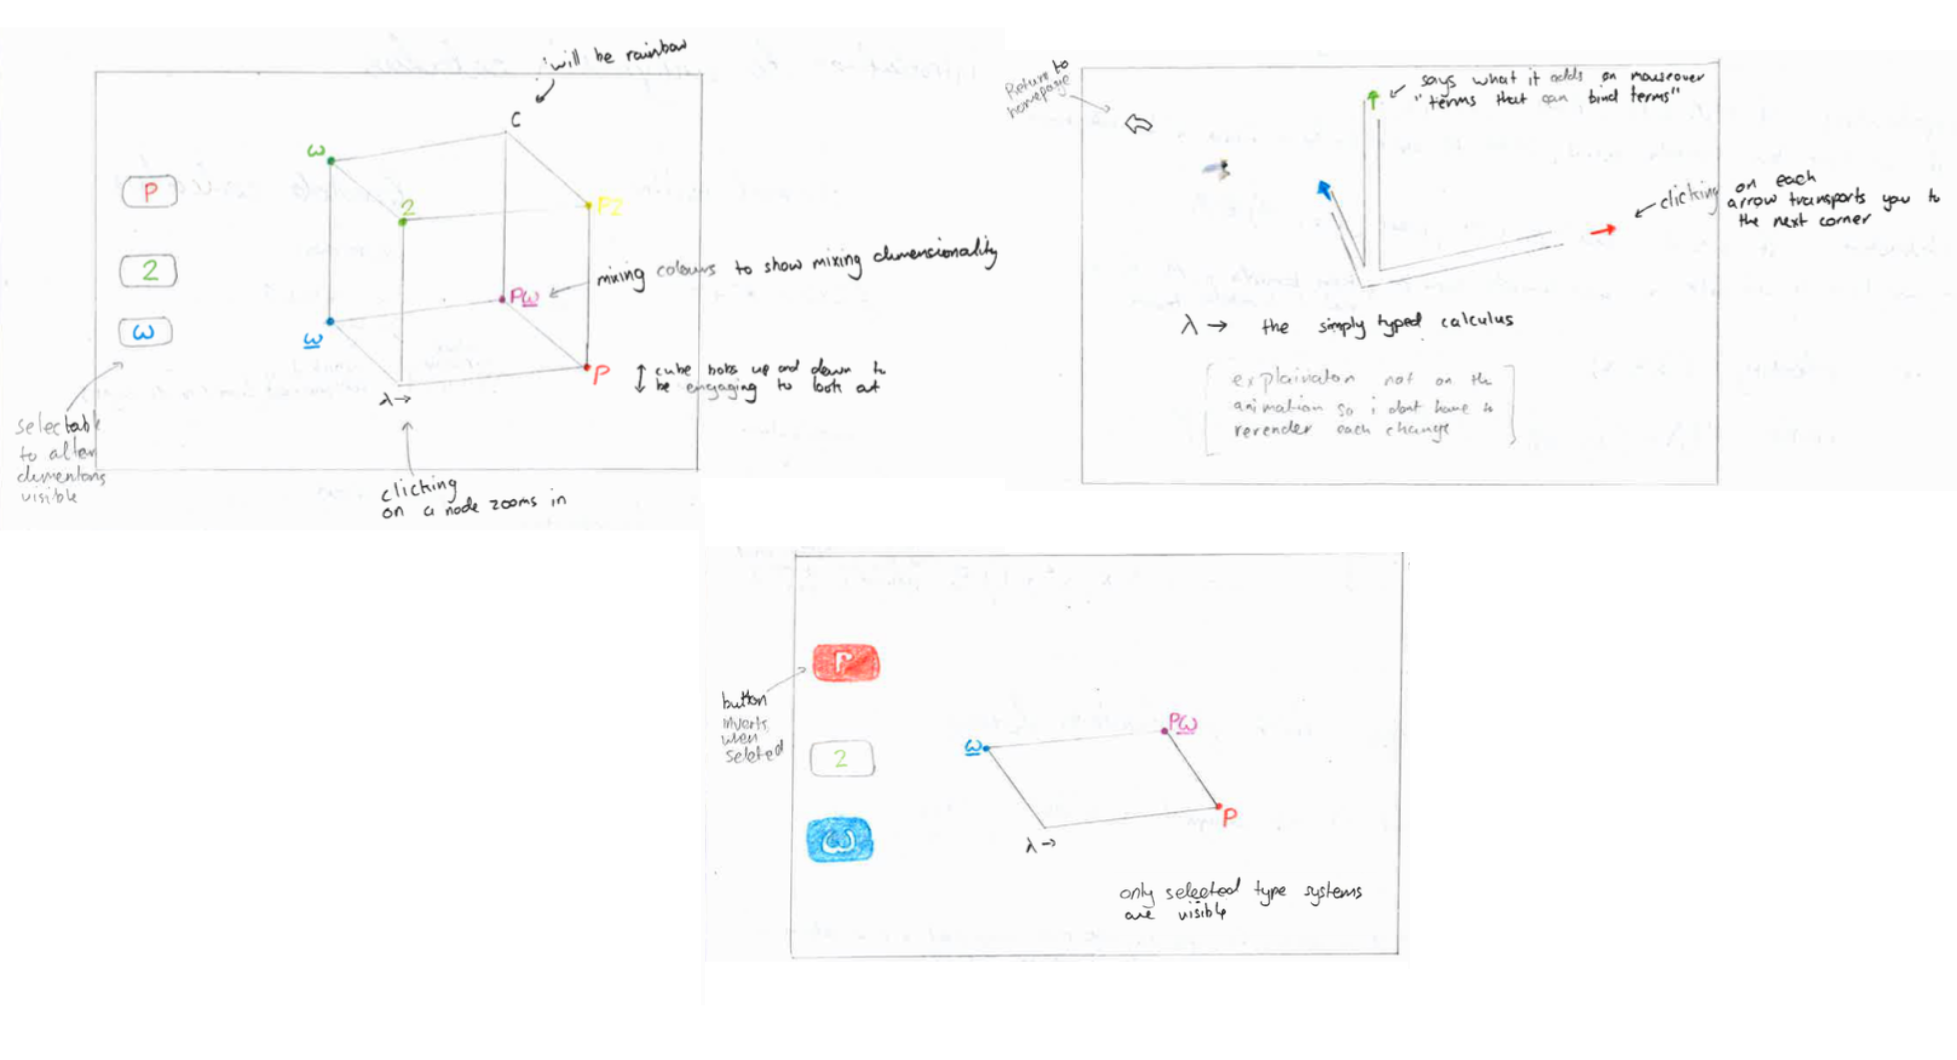
\includegraphics[width=1\linewidth]{dissertation/images/paper_collaged_taller.png}
    \caption{A scan of my final paper sketch ideas}
    \label{fig:enter-label}
\end{figure}

The (collaged) scan shows the thee main states that I planned for my website to have.  The top left shows the home page in the normal state when you open the website.  This has a diagram of the cube, with the corners labeled in the colours derived by mixing those I assigned to the axes.  I also included notes that the cube should constantly moving a little bit.  I decided to do this so that the page would not look as boring and static, which would hopefully aid in keeping the user's attention.  

There are also three buttons on the left side of the screen.  I planned to have these as a way of removing type systems from the cube, so that there would be only a line or square if one or two buttons were selected respectively.  This could be used to narrow down the amount of information presented on the screen at any one time, to avoid overwhelming a new user by narrowing down the potential options available to them.  This would also let an experienced user refine their use to only show relevant information.
\pagebreak

After this, I transitioned to using Figma to further develop my design.  I chose to use Figma because I was already familiar with the technology from the third year team project.  Figma is better to use at this stage of the project as it allows you to undo and redo actions, as well as copy and paste similar elements, which cannot be done with pen and paper.

\begin{figure}[h!]
    \centering
    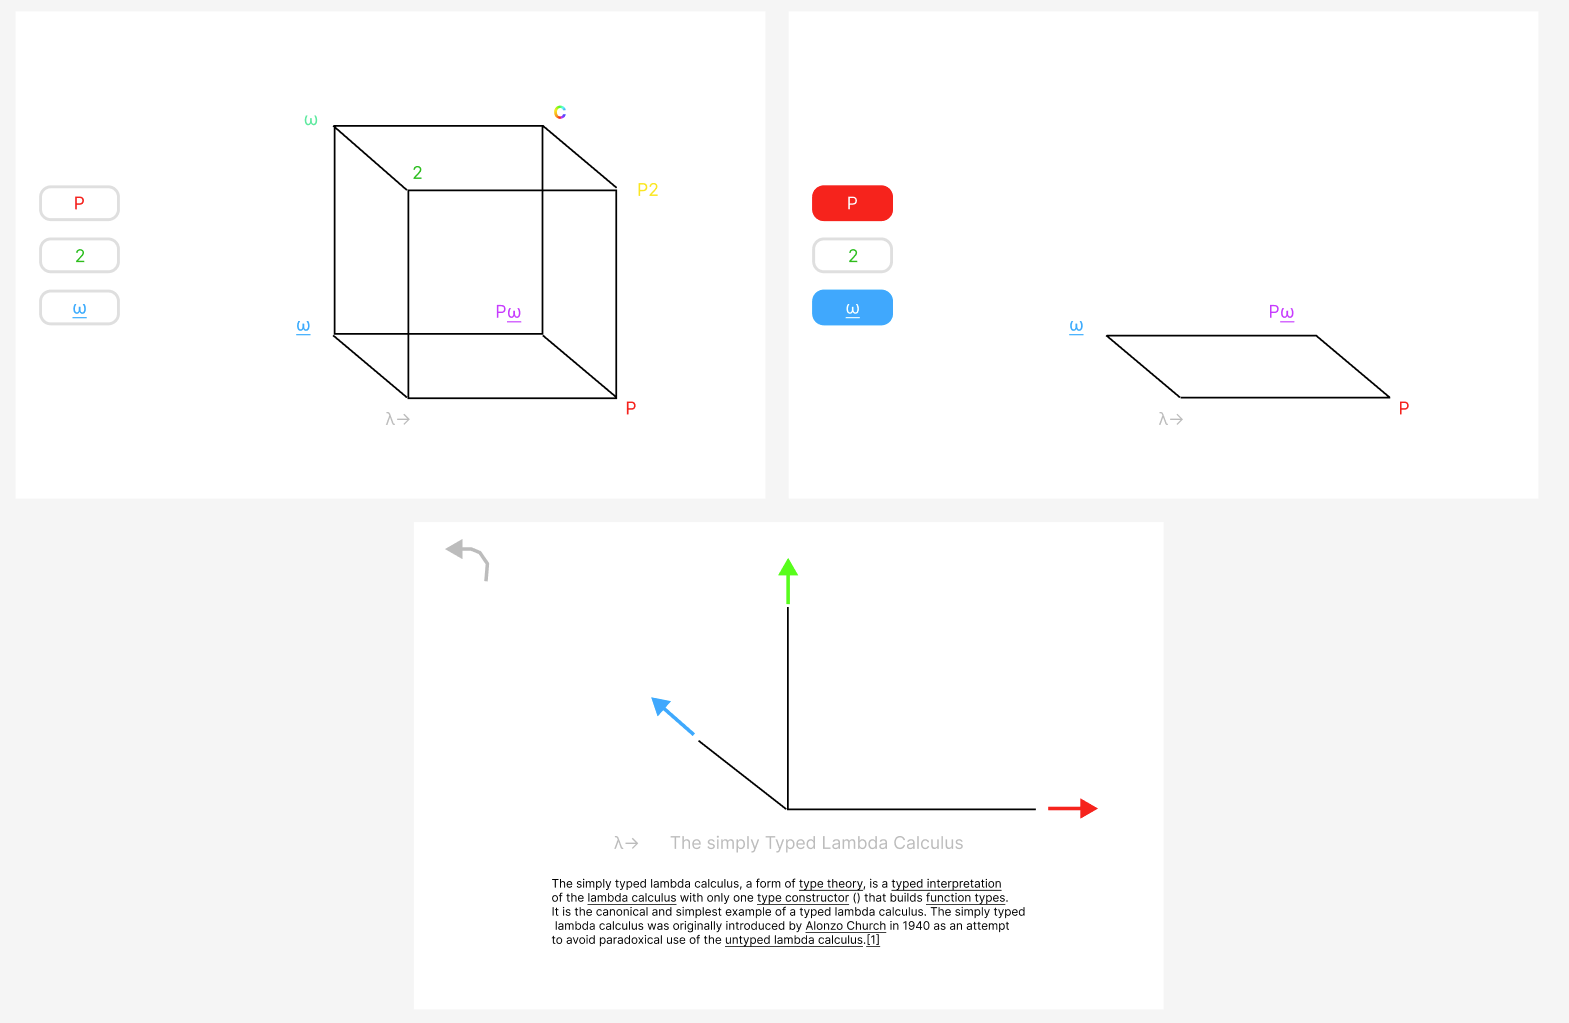
\includegraphics[width=1\linewidth]{dissertation/images/v1_full_taller.png}
    \caption{A screenshot of the first Figma version}
    \label{fig:enter-label}
\end{figure}

While refining my design in Figma, I decided to delete the function to show and hide dimensions, as it did not seem useful.  I concluded that it did not offer more functionality than clicking on a single node, or just looking at one dimension at a time using the arrows.  As well as this, it could be seen as confusing to some users, who might not understand the concept or could remove a dimension and forget to re add it later, locking them out of learning more

I repurposed the side button elements into buttons which move you to a different node instead.  I also decided to put the page contents into text boxes that I would position around the screen, instead of being in one scrollable section in the middle.  I chose to make this change after having to constantly scroll up and down in papers to read different sections, and noticed that this could be largely eliminated by making better use of the empty space in and around the cube.

\begin{figure}[h!]
    \centering
    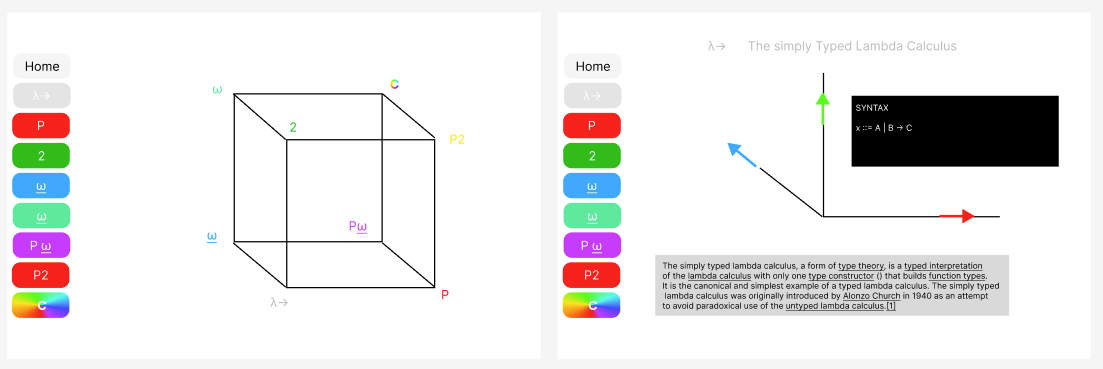
\includegraphics[width=1\linewidth]{dissertation/images/v2_full.png}
    \caption{A screenshot of the final Figma version}
    \label{fig:enter-label}
\end{figure}

\section{Research}

The greatest struggle I had during the design phase of my project was researching and finding sources for the different systems.

P2

P Weak omega


%==================================================================================================================================
\chapter{Implementation}


\section{Using WebGL}

poorly documented

'the Book of Shaders'

lerp

\section{Using Elm}

What my model looks like

The messages that I have

How my file structure is set out

\section{LaTeX2Elm Translator}

\section{Portability}

Browser portability

screen resolution

\section{Summary}


%==================================================================================================================================
\chapter{Evaluation} 

\section{Evaluating Based on University Accessibility Guidelines}

\section{Experiment Methodology}

In order to assess how effective my website was at teaching people concepts from the lambda cube, I ran a set of user studies on students who were already familiar with some basic concepts of programming languages.  I chose this subset as they are the primary intended audience for the website once it is launched, and if I used people who were totally unfamiliar with the concept of lambda calculus then they could spend too long learning the basics at the untyped lambda calculus node to effectively have time to explore the cube itself.

The study I planned to run was split into two parts.  First the user would be given 15 minutes to use the website, while I observed and made notes on how they used it.  Then the user would be given a questionnaire to fill out without using the website.  The questionnaire had four sections:

\begin{itemize}
    \item First, the user would be asked to rank them self based on their confidence in three different areas of prior knowledge: Knowledge about lambda calculus, Familiarity with BNF syntax and familiarity with formal logic.  By collecting this data, I would have enough background about each student to be able to draw conclusions from their results in the next parts of the survey.

    \item Next, they would be given a wireframe of the lambda cube and of it's axes, and be asked to label the corners of the cube and the type systems represented by the axes.  This is the most basic information about the lambda cube, so by giving them a simple recall task I would be able to tell how effective the website is at teaching the fundamental concepts of the cube.

    \item After this, the respondent is given three more complex recall questions, asking about specific features of some of the systems, and giving them a few lines to write an answer to each.  By having some longer questions about deeper topics, I could see how effectively my website is able to express more complex aspects of the lambda cube.

    \item Finally, there is a section where the user is directly asked for feedback, both by ranking the site in terms of legibility, information quality, information depth, feature richness and aesthetics, and a section where they were free to write any feedback or suggestions they had.  By having both of these two sections, I could gather quantitative and qualitative feedback, diversifying the types of feedback I could use.
\end{itemize}

\section{Study Results}

TABLE WITH RESULTS

\section{Changes I made}

Guided tour mode \& reorganised sidebar

While the gentle movement of the cube was generally well received, some users also reported that the animation was distracting or slightly nauseating.  As a result I decided to add in an option to pause the cube's movement indefinitely.  This is achieved using a media query to search the computers settings to find if the user has 'reduced-motion' turned on, and using a port to set this value in the local library.  This value was then passed into the main function of my elm program with the flags, where it could be changed with the press of a button.

One of the students who I surveyed was red-green colourblind, and as a result was less able to distinguish between the Polymorphic types and Dependent types.  In order to accommodate users with similar accessibility requirements, while keeping the same aesthetic that was liked by by the other users, I chose to implement a selectable colour blind mode.  This would be a button placed next to the reduced motion button which would toggle between the base state, using the same colours as before, and a mode which changes all of the colours to safe versions which can be more easily distinguished by users who are colourblind or otherwise visually impaired.

I then used the HTML With context package to 

An advantage of this approach was that this solution is readily scalable

\section{Conclusions}

My user studies were very useful for helping me find deficiencies in my website that I could not notice.  This was my main focus going into the studies, and I found the observation and questionnaire worked very well at helping me to notice areas where I could improve my website

The scores for the test sections of the study were universally quite low.  This could be because everyone surveyed had taken programming languages last year, so had forgotten a lot of the relevant information, or 

The study however was not useful to find out if my website was more effective than the other options, as I gathered no data to compare mine to.

I should have instead split my study group into two sections, with one completing the same questions about the Wikipedia page I was using as a bench mark, and the other group to use my website.  By A/B testing the websites against each other, I would be able to draw statistically valid conclusions about the efficacy of my attempt to improve upon previous attempts.  This would be more effective than reusing the same group on both websites back to back, as it would mean that the users would be able to go into both experiences fresh, and the knowledge gained during the first trial would not effect their performance during their second one. 

However, this would effectively half my sample size, which was already rather small, so any conclusions that I may have been able to draw not have been statistically valid either way.

%==================================================================================================================================
\chapter{Conclusion}    

\section{Summary}

I used Elm as the basis for my website, and WebGL to create a cube that could be rendered and have its orientation changed in real time to render the lambda cube in real time.

My main design problems were finding ways to display the information consistently.

In order to depict the BNF syntax, I had to create a translator, using Deno, which takes a .tex file of an equation and returns a .elm file which can easily be rendered

After my user studies, I focused on the user experience, and making the website more accommodating to a wide range of users

\section{Reflection}

I should have used a more structured timeline of tasks

Researching and finding sources proved to be one of the most difficult parts of the whole process

I am very happy with my choice of elm \& the website I was able to create using it

I should have run different tests to validate my project, and struggled to find a suitable and large enough sample size

\section{Future Work}

Screen reader accessibility

Edit suggestion framework to make the project collaborative

%==================================================================================================================================
%
% 
%==================================================================================================================================
%  APPENDICES  

\begin{appendices}

\chapter{Appendices}

Typical inclusions in the appendices are:

\begin{itemize}
\item
  Copies of ethics approvals (required if obtained)
\item
  Copies of questionnaires etc. used to gather data from subjects.
\item
  Extensive tables or figures that are too bulky to fit in the main body of
  the report, particularly ones that are repetitive and summarised in the body.

\item Outline of the source code (e.g. directory structure), or other architecture documentation like class diagrams.

\item User manuals, and any guides to starting/running the software.

\end{itemize}

\textbf{Don't include your source code in the appendices}. It will be
submitted separately.

\section{Task Sheet for User Evaluation}

\section{User Evaluation Results}

\end{appendices}

%==================================================================================================================================
%   BIBLIOGRAPHY   

% The bibliography style is abbrvnat
% The bibliography always appears last, after the appendices.

\bibliographystyle{abbrvnat}

\bibliography{l4proj}

\end{document}
